\documentclass[10pt, oneside]{article}
\usepackage{amsmath, amsthm, amssymb, calrsfs, wasysym, verbatim, bbm, color, graphics, geometry}
\usepackage{graphicx}
\graphicspath{ {./assets/} }
\geometry{tmargin=.75in, bmargin=.75in, lmargin=.75in, rmargin = .75in}

\newcommand{\R}{\mathbb{R}}
\newcommand{\C}{\mathbb{C}}
\newcommand{\Z}{\mathbb{Z}}
\newcommand{\N}{\mathbb{N}}
\newcommand{\Q}{\mathbb{Q}}
\newcommand{\Cdot}{\boldsymbol{\cdot}}

\newtheorem{thm}{Theorem}
\newtheorem{defn}{Definition}
\newtheorem{conv}{Convention}
\newtheorem{rem}{Remark}
\newtheorem{lem}{Lemma}
\newtheorem{cor}{Corollary}
\usepackage{biblatex} %Imports biblatex package
\addbibresource{reference.bib} %Import the bibliography file

\title{Summary Report: The threshold effect of institutional quality on sovereign debt and economic stability}
\author{Alejandro Ouslan}
\date{2025-04-16}

\begin{document}

\maketitle
\tableofcontents

\vspace{.25in}

\section{Summary}
The paper "Threshold Effects of Inequality on Economic Growth in the US States:"\cite{ccepni2020threshold} look to find the effects of inequality
on the economic growth of the US states. Key points:
\begin{itemize}
	\item At first physical capital is higher relative to that on human capital, but in later stages this is flipped
	\item
\end{itemize}

\section{Data sources}

\section{Methodology}
\begin{itemize}
	\item They use a theoretical frame work of Galor and Moav \cite{moav2004physical}
	\item The study make use of 48 states from 1948 to 2014.
	\item The dependent variable of Growth is the annual growth rate of real per capita state income. (BEA)
	\item They deflated the data using the CPI from the FRED database.
	\item From FRED they also obtained the GINI
	\item Their model que be summarize ice in the following formula:
	      \begin{equation}
		      y_{it} = \mu_i + \beta_2 x_{it} I(q_{it} \le \gamma) + \beta x_{it} I(q_{it} > \gamma) + \theta' z_{it} + e_{it}
	      \end{equation}
	      \begin{itemize}
		      \item $I(\cdot)$ is an indicator function
		      \item $q_{it}$ is the threshold variable (HKC or HKH),
		      \item $\gamma$ is the threshold parameter that divides the equation into different regimes
		      \item $z_{it}$ is the set of growth determinants (LY0, POPG, HKH or HKC)
		      \item $x_{it}$ is the measure of income inequality (GINI).
		      \item $e_it$ is the error term $e_it \sim N(0,\sigma^2)$
	      \end{itemize}
	\item Their Hypothesis is threshold effects
	      \[
		      \begin{split}
			      H_0 & : \beta_i = \beta_2    \\
			      H_1 & : \beta_1 \neq \beta_2
		      \end{split}
	      \]
	\item the leas square estimator of parameter $\gamma$ is obtained by:
	      \begin{equation}
		      \hat{\gamma} = argmin S_1(\gamma)
	      \end{equation}
	      item their F-statistic is contracted as:
	      \begin{equation}
		      F_1= \frac{S_0 - S_1(\gamma)}{\hat{\sigma^2}}
	      \end{equation}
\end{itemize}

\section{Results}
\begin{figure}[h]  % 'h' forces the figure to be placed here, if possible
	\centering
	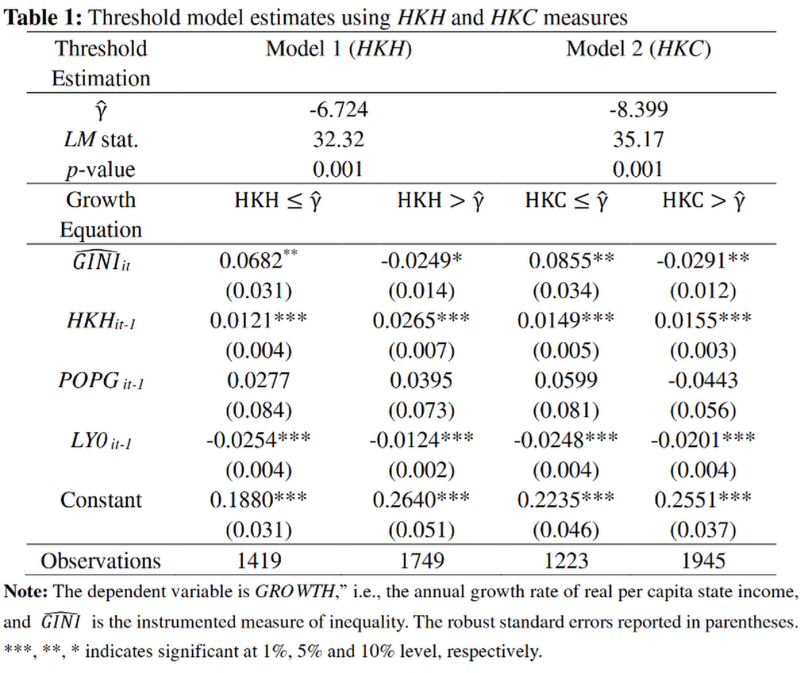
\includegraphics[width=\textwidth]{table_1.png}  % Adjust the width as needed
	\caption{Caption for Table 1}
\end{figure}


\section{Conclusions}
The conclusions are as follow:
\begin{enumerate}
	\item This model tend to suggest that while the effect is positive below
	      a certain threshold of the ratio of human to physical capital,
	      the effect turns negative thereafter
	\item analysis shows that while the effect of inequality on growth is significantly positive at
	      lower levels of development, this effect turns significantly negative at higher levels of
	      development
\end{enumerate}
\cite{ccepni2020threshold}
\printbibliography
\end{document}
